\documentclass[usenatbib]{mn2e} 
\usepackage{amsmath} 
\usepackage{amssymb} 
\usepackage{graphics}
\usepackage{graphicx}
\usepackage{epsfig} 
\usepackage{float} 
\def\be{\begin{equation}}
\def\ee{\end{equation}}
\def\ba{\begin{eqnarray}}
\def\ea{\end{eqnarray}}
\bibliographystyle{mn2e}
% To highlight comments 
\usepackage{color}
\definecolor{red}{rgb}{1,0.0,0.0}
\newcommand{\red}{\color{red}}
\definecolor{blue}{rgb}{0.1,0.3,0.9}
\newcommand{\blue}{\color{blue}}

\usepackage[normalem]{ulem}
\definecolor{darkgreen}{rgb}{0.0,0.5,0.0}
\newcommand{\SRK}[1]{\textcolor{darkgreen}{\bf SRK: \textit{#1}}}
\newcommand{\SRKED}[1]{\textcolor{darkgreen}{\bf #1}}

\newcommand{\LCDM}{$\Lambda$CDM~}
\newcommand{\beq}{\begin{eqnarray}}  
\newcommand{\eeq}{\end{eqnarray}}  
\newcommand{\zz}{$z\sim 3$} 
\newcommand{\apj}{ApJ}  
\newcommand{\apjs}{ApJS}  
\newcommand{\apjl}{ApJL}  
\newcommand{\aj}{AJ}  
\newcommand{\mnras}{MNRAS}  
\newcommand{\mnrassub}{MNRAS accepted}  
\newcommand{\aap}{A\&A}  
\newcommand{\aaps}{A\&AS}  
\newcommand{\araa}{ARA\&A}  
\newcommand{\nat}{Nature}  
\newcommand{\physrep}{PhR}
\newcommand{\pasp}{PASP}    
\newcommand{\pasj}{PASJ}    
\newcommand{\avg}[1]{\langle{#1}\rangle}  
\newcommand{\ly}{{\ifmmode{{\rm Ly}\alpha~}\else{Ly$\alpha$~}\fi}}
\newcommand{\hMpc}{{\ifmmode{h^{-1}{\rm Mpc}}\else{$h^{-1}$Mpc }\fi}}  
\newcommand{\hGpc}{{\ifmmode{h^{-1}{\rm Gpc}}\else{$h^{-1}$Gpc }\fi}}  
\newcommand{\hmpc}{{\ifmmode{h^{-1}{\rm Mpc}}\else{$h^{-1}$Mpc }\fi}}  
\newcommand{\hkpc}{{\ifmmode{h^{-1}{\rm kpc}}\else{$h^{-1}$kpc }\fi}}  
\newcommand{\hMsun}{{\ifmmode{h^{-1}{\rm {M_{\odot}}}}\else{$h^{-1}{\rm{M_{\odot}}}$}\fi}}  
\newcommand{\hmsun}{{\ifmmode{h^{-1}{\rm {M_{\odot}}}}\else{$h^{-1}{\rm{M_{\odot}}}$}\fi}}  
\newcommand{\Msun}{{\ifmmode{{\rm {M_{\odot}}}}\else{${\rm{M_{\odot}}}$}\fi}}  
\newcommand{\msun}{{\ifmmode{{\rm {M_{\odot}}}}\else{${\rm{M_{\odot}}}$}\fi}}  
\newcommand{\lya}{{Lyman$\alpha$~}}
\newcommand{\clara}{{\texttt{CLARA}}~}
\newcommand{\rand}{{\ifmmode{{\mathcal{R}}}\else{${\mathcal{R}}$ }\fi}}  
\newcommand{\hs}{{\hspace{1mm}}}  
\newcommand{\kms}{\,km~s$^{-1}$}

% definition to produce a "less than or similar to" symbol
\def\lsim{~\rlap{$<$}{\lower 1.0ex\hbox{$\sim$}}}

% definition to produce a "greater than or similar to" symbol
\def\gsim{~\rlap{$>$}{\lower 1.0ex\hbox{$\sim$}}}

\begin{document}

\title[Rotation in the Lyman-$\alpha$ line]{Rotation effects on the
  Lyman-$\alpha$ line morphology in distant galaxies}
\author[Garavito-Camargo, Forero-Romero \& Dijkstra]{
\parbox[t]{\textwidth}{\raggedright 
  Nicolas Garavito-Camargo$^{1}$,
  Jaime E. Forero-Romero$^{1}$ and 
  Mark Dijkstra$^2$
}
\vspace*{6pt}\\
$^{1}$Departamento de F\'{i}sica, Universidad de los Andes, Cra. 1
No. 18A-10, Edificio Ip, Bogot\'a, Colombia \\
$^2$
}
\maketitle

\begin{abstract}
Rotation is present in the gas kinematics of galaxies up to the
highest redshifts. In this paper we present for the first time
radiative transfer calculations that show the impact of rotation on
the morphology of the Lyman $\alpha$ line. To this end we construct
simplified models where a galaxy is modeled as an homogeneous sphere
composed as an homogeneous mixture of dust and hydrogen at a constant
temperature. These spheres have a solid-body rotation with linear
velocities at the surface in the range $0-300$ \kms. We consider
radiation sources both in the center of the rotating cloud and also
homogeneously distributed around the sphere. We find that higher
rotational velocities increase the width of each peak in the outgoing
line profile while it also increases the amount of Lyman alpha photons
escaping in the line center. This trends makes that for high
rotational velocities and large Hydrogen optical depths the double
peak of the line tends to be erased an be replaced by a single peak the
lines center. This is more pronounced for radiation sources
homogeneously distributed. Concerning the escape fraction we find that
rotation does not have any effect, provided that all the sources are
centrally emitted. However in the case of homogeneously emitted
sources we measure an increase of about a factor of $2$ in the escape
fraction for higher rotational velocity values. 
Our work shows clearly that gas rotation has a non negligible impact
on the shape of the Lyman $\alpha$ line. 
\end{abstract}
\begin{keywords}
galaxies: high-redshift - galaxies: star formation - line: formation
\end{keywords}


\section{Introduction}
\label{sec:intro}



Due to the resonant nature of the Lyman alpha line, gas kinematics
play an important role shaping its morphology...

There is an extensive literature studying the influence of
outflow/inflow configurations in the shape of the outgoing Lyman-alpha
line...

In this paper we study for the first time the impact of rotation on
the morphology of the Lyman $\alpha$ line. To isolate the effects of
rotation we focus on a simple system: the gas distribution is
spherical, with homogeneous density and the gas rotates as a solid
body. We base our work on two independent Monte Carlo based radiative
transfer codes CLARA \citep{CLARA} and XX \citep{DijkstraKramer}.

 
This paper is paper is structured as follows...

In this paper we express a photon's frequency in terms of the
dimensionless variable $x\equiv (\nu -\nu_a)/\Delta\nu_\alpha$, where
$\nu_{\alpha}=2.46\times 10^{15}$ Hz is the Ly$\alpha$ resonance
frequency,  $\Delta_{\alpha} \equiv
\nu_{\alpha}\sqrt{2kT/m_pc^2}\equiv \nu_av_{\rm th} $ is the doppler
broadening of the line which depends on the neutral gas temperature
$T$ scattering the radiation or equivalently the thermal velocity
$v_{\rm th}$ of the atoms.


\section{Modeling Bulk Gas Rotation}
\label{sec:implementation}

Describing the kinematics of gas rotation in all generality is a
complex task. There is great variation in the shape of the rotation
curve as observed in HI emission as a function of the distance to the
galaxy center. However there are two features that are observed very
often. First, in the central region the velocity increases
proportional to the radius following the behaviour in a body with
solid rotation. Second, beyond a certain radius the rotation curve
tends to flatten. Furthermore, a thorough observational account of gas
rotation in the redshifts of interest for the study of LAEs ($z>1.0$)
is still missing. 


An ab-initio description of realistic rotation curves in simulations
depends on having access to the dynamic evoluction the mass components
in the galaxy: stars, gas and dark matter. Such level of realism is
extremely complex to achive, specially of one wants to get a
systematic description based on statistics of simulated objects.


Following the tradition of studies of Lyman$\alpha$ emitting systems,
we implement a model with a simplified geoemtry and gas
distribution. We assume that the gas is homogeneously distributed in a
sphere that rotates as a solid body with constant angular
velocity. This simple model will contain only one parameter: the
linear velocity at the sphere's surface, $V_{\rm max}$.

\subsection{Detailed Implementation of Rotation}

 In the MonteCarlo code we define a cartesian coordinate system to
 define the position of each photon. The origin of this system
 coincides withthe center of the sphere and the rotation axis is defined
 to be $z$-axis. With this choice, the components of the gas bulk velocity
 field, $\vec{v} = v_{x}\hat{i} + v_{y}\hat{j} + v_{z}\hat{k}$, can be
 written as  
  
\begin{subequations}
\begin{align}
    v_{x}=-\dfrac{y}{R}V_{\rm max}, \label{subeq1}\\
    v_{y}=\dfrac{x}{R}V_{\rm max}, \label{subeq2}\\
    v_{z}=0, \label{subeq3}
\end{align}
\end{subequations}
%
where $R$ is the radius of the sphere and $V_{\rm max}$ is the linear
velocity at the sphere's surface. The minus/plus sign in the
$x$/$y$-component of the velocity indicates the direction of
rotation. In this case we take the angular velocity in the same
direction as the $\hat{k}$ unit vector. With these definitions we can
write the angular velocity as $\omega=V_{\rm max}/R$.  

In contrast with spherically symmetric models (static, outflow,
inflow) the rotation now defines a preferred direction in the
problem. In Section \ref{sec:results} we quantify this differences by
varying the line of sight of a mock observer with respect to the
rotation axis. The results are parameterized by the polar angle
$\theta$ as defined by the dot product $\cos\theta =
{\hat{u}\cdot\hat{k}}$. 

\subsection{Grid of Simulated Galaxies}
\label{sec:models}

In the Monte Carlo calculations we follow the propagation of $N_{\gamma}=10^5$
numerical photons through different spherical galaxies, each one
varying in at least one of the following parameters: the maximum
rotational velocity $V_{\rm max}$, hydrogen optical depth $\tau_{H}$,
dust optical depth $\tau_{a}$ and the initial disitrbution of photons
with respect to the gas. There are in total 60 models with the input
parameters summarized in Table \ref{table:models}.  

\begin{table}
\begin{center}
\begin{tabular}{llc}\hline\hline
Physical Parameter (units) & Symbol & Values\\\hline
Velocity (\kms) & $V_{\rm max}$&$0,\ 50,\ 100,\ 200,\ 300$\\
Hydrogen Optical Depth & $\tau_{H} $ & $10^{5},\ 10^{6},\ 10^{7}$\\
Dust Optical Depth & $\tau_{a}$ & $0$,$1$\\
Photons Distributions & & Central, Homogeneous\\\hline\hline
\end{tabular}
\caption{
List of the physical parameters that define the spherical models we
have simulated using Monte Carlo calculations. For each parameter we
vary the values in the range listed in the last column. Takig into
account all the possible combinations we end up with $60$ different
models. } 
\label{table:models}
\end{center}
\end{table}


\section{Results}
\label{sec:results}

The central result of this paper is summarized in
Fig.~\ref{fig:differentvelocities} that shows clearly the considerable
impact of rotation on the morphology of the emergent \ly line. Both
panels in the Figure focus on the results for $\tau_{H}=10^{7}$,
showing that the influence of rotation is present both when the
photons are either homogeneusly or centrally initialized over the gas
volume. 

These results for these outgoing spectra are constructed by taking into
account all outgoing photons regardless of the direction of
propagation. In subsection \ref{subsec:direction} we report different
statistics aiming at quantifying the changes in the observed spectra
for observers with different viewing angles.



\begin{figure*}
  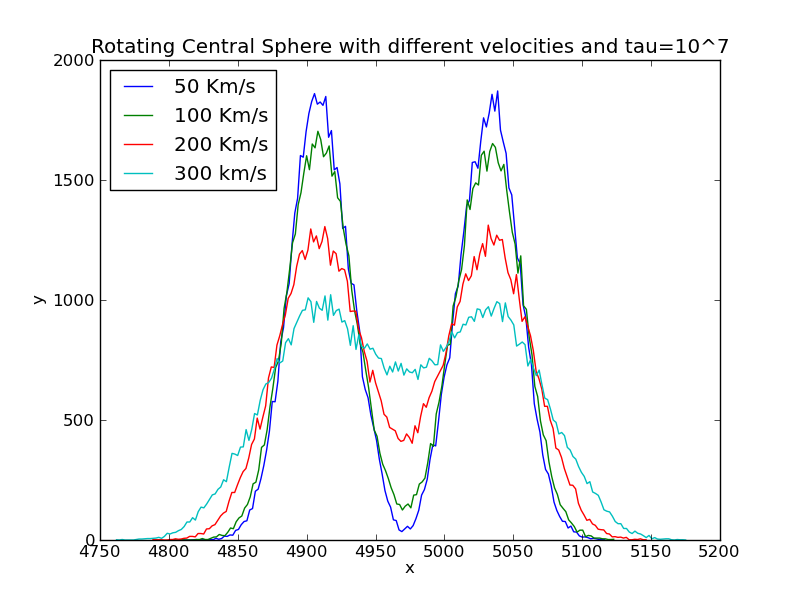
\includegraphics[width=0.45\textwidth]{7tDifSpeedsZ.png}
  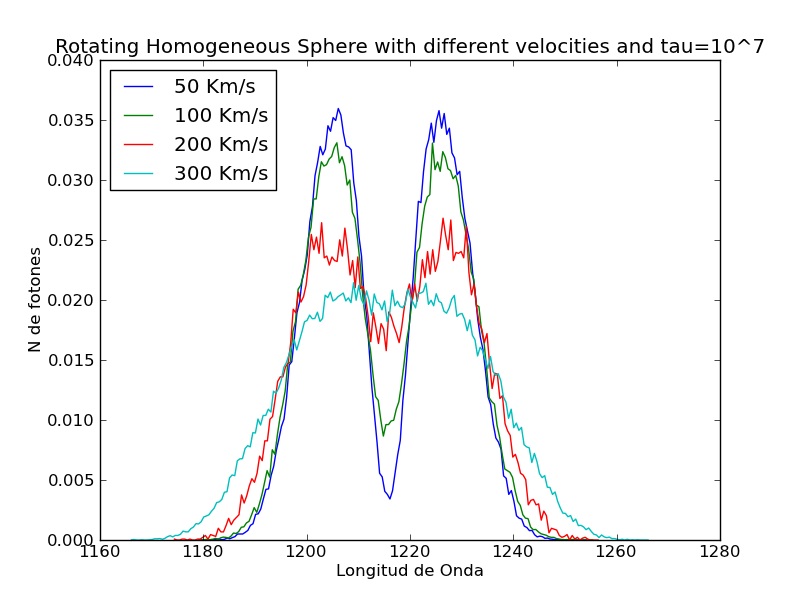
\includegraphics[width=0.45\textwidth]{7tHOMDifSpeeds1.png}
\caption{Shape of the lyman alpha line for
    different velocities. The left (right) panel shows the central
    (homogeneous) photon distribution. All photons were taken into
    account regardless of their outgoing direction of propagation.
  \label{fig:differentvelocities}}
\end{figure*}

In the following subsections we quantify the trends observed in
Fig. \ref{fig:differentvelocities} and
Fig. \ref{fig:differentobservers} as a function of the maximum
rotation velocity $V_{\rm max}$ and the position of the observer with
respect to the rotation angle, $\mu = \cos{\theta}$. All the results
in this section will be expressed in terms of the adimensional
frequency $x$.

First we quantify the line by its full width at half maximum
(FWHM) and the peak positions. In order to interpret these results we
measure how the rotation affects the average number of scatterings
for each Lyman-alpha photon in the simulation. This help us to
introduce the next subsection on the escape fraction in our models
including dust. We conclude the section by estimating the
expected line flux for top hat filters at a fixed center and varying
width. 

\subsection{Line width and peak maxima}
\label{sec:widthpeak}
\label{fig:differentvelocities}

\begin{figure}
    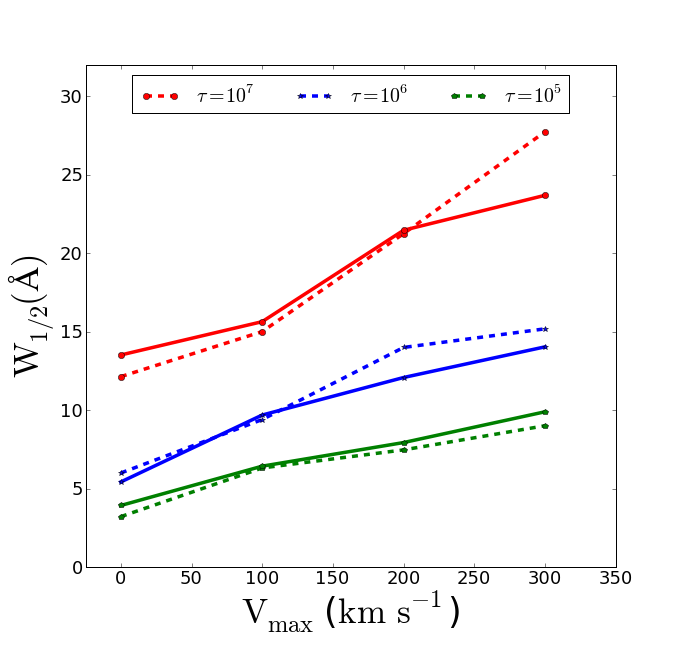
\includegraphics[width=0.45\textwidth]{WidthvsVmax.png}
\caption{Width of the lyman-alpha line for all the models.\label{fig:widthvsvelocity}}
\end{figure}


The first quantitative conclusion of the effect of rotation in the
Lyman alpha line is that the double peaks in the line tend to broaden
until they reach a single broad emission peak. This is most evident in
the case of Lyman-alpha sources homogeneously distributed in the gas
distributions (Fig.~\ref{fig:differentvelocities} Right panel).

To quantify the line broadening we measure a modified version of the full
width at half maximum (FWHM) for half of the line, $W_{1/2}$. It means that in
the case of double peaked emission, $W_{1/2}$ corresponds to the with
one of the peaks, while in the extreme case when the line is converted
into a single peak, $W_{1/2}$ corresponds to half of the full width. 

This definition allows us to quantify the line width both in the cases
of double and single peak emission. Furthermore it has the advantage
that this line width should have a direct observational correspondence
to the observed line feature once the Inter-Galactic Medium (IGM)
effects are taken into account, which have the central effect of
strongly reducing the intensity of the blue peak of the line.

Fig.~\ref{fig:widthvsvelocity} summarizes our findings for $W_{1/2}$
as a function of $V_{\rm max}$. The line width increases with the
rotational velocity of the gas cloud. This increase can be of a factor
of $2-3$ with respect to the width with respect to the static
case. This trend is conserved at all optical depths regardless of the
initial source distribution. 

%Im not sure about this anymore---TALK to Jaime about this!
This result includes all the outgoing photons, regardless of the
position of the observer. In Figure~\ref{fig:widthvstheta} we
take into account the different positions of the observer in the
measurement of the half-width $W_{1/2}$. From this we conclude
that observers with a line of sight perpendicular to the axis of
rotation (i.e. edge-on in the case of spiral galaxy) tend to measure
larger line widths than observers aligned with the rotation axis
(i.e. face-on). The influence of the observer position on the line
width, amounting always less than $15\%$ of a difference with respect
to the result that takes into account all the outgoing photons with
the same weight regardless of the relative observer position.

%Both for central and homogeneous distribution of sources, We found a
%dependency of the width with the rotation velocity of the gas cloud,
%this results are summarize in Figure ~\ref{figure:width}. As velocity
%increase also the equivalent width increase (for both homogeneous and
%central distribSi Limonution), it means that some photons escape with fewer
%scatterings than the static case but at the same time a few photons escape with% more scatterings, this can be seen clearly in
%Figure. (Nscatt)\\ 

%We also found a dependency with the viewing angles, in particular as
%the angle incre ase the width also increase Figure
%~\ref{fig:withvstheta}, this was also found in Verhemme et al. 2012
%for a rotating disk but the pure effect of rotation can not been study
%as it is in our case. Following the convention of Verhamme et al 2012
%we define $\mu=cos(\theta)$, and we can make a polynomial fit for the
%$FWHM(\mu)$ for our models, this is resumed in Table ~\ref{table:fits} 


\begin{figure}
    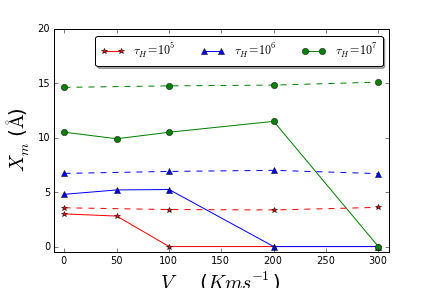
\includegraphics[width=0.45\textwidth]{maximumvsVmax.png}
\caption{Position of the maxima
    in the outgoing spectra for differents Rotational velocities,
    (up)Central Distriution, (Down) Homogeneous Distribution.\label{fig:maximumsvsvelocity}} 
\end{figure}

The second feature in the line that we use to quantify the effect of
rotation is the position of the line maxima. These provide information
on the wavelength of the majority of the outgoing photons after
they interact with the neutral hydrogen atoms in the gas cloud. If
most of the photon escapes with a low number of scattering, its
outgoing frequency will be close to its initial frequency, that is in
the center of the line. On the contrary if the number of scatterings
is large for the average photon, its outgoing frequency will be far
from the line center. Such reasoning can be made more quantitative to
understand the dependence of the peak maxima as a function of the
hydrogen optical depth in the cloud [citation needed].


In Fig.~\ref{fig:maximumsvsvelocity} we present the position
of the maxima as a function of $V_{\rm max}$. For the photons emitted
in the line center we do not find any variation in the position of the
maxima in the range of explored parameter space (dash lines). However in the
homogeneous case we can see how the maxima goes to $x_{m}=0$, meaning
that the double peak is converted into a single peak.

This transition to a single peak line occurs for the systems where it
becomes easier for a bulk of the photons to escape with the lowest
number of scatterings possible. This can explain how the single peak
stage can be achieved in the homogeneous source distribution where
there is fraction of the photons inside a photosphere region with
$\tau_{H}\sim 1$ which allows them to escape within one
scatter. Increasing the rotational velocity makes it easier for the
photons in this photosphere region to escape.

We also take into account the viewing angle $\mu$ for all the optical 
depths and rotational velocities and the two different photon distribution.
But we don't find any dependency meaning that the peaks would be placed in
the same place no matter the position of an external observer.	

Finally we also report on the effect of the neutral Hydrogen
optical depth $\tau_{H}$ on the maxima position $x_{m}$
Fig.~\ref{fig:maximumsvsvelocity}. We find that, at fixed
rotation velocity, the position of the maxima increases with optical
depth as expected from basic theoretical considerations. We compare
our results with the expected theoretical scaling for an infinite
slab. 



\subsection{Average Number of Scatterings}

Until know we have focus in how rotation affect the morphology of the 
Lyman alpha line, now we turn to study deeply the possible causes of 
this effects. As recombination is the main cause of the emission of the 
Lyman alpha line, it is important to study the relationship between the 
number of times that a photon is absorbed and re emitted that we simply 
take as scatterings with it's shift in the wavelength. 

As a first approach we study the number of scatterings of all the photons 
at different velocities and for both photon distributions Figure~\ref{fig:Nscatt}. 
For the central distribution we found that the average number of scattering 
does not have a relevant change ($\sim 0.5\%$) with $V_{max}$, For the 
Homogeneous distribution we found that as $V_{max}$ increase the average 
number of scatterings decrease in a$\sim 39\%$, it means that rotation 
makes photons to escape easier from the cloud. The reason why this is not 
observed in the central distribution is because the amount of gas that every 
photon has to break through is so large that the average number of scatterings 
is large too, making the effect of rotation unobservable.

In order to understand the effects of rotation in the morphology of the line
 we make histograms of $<N_{scatt}>$  in function of $X_{m}$ for both the 
 central Fig.~\ref{fig:NscattHisto} and the  homogeneous distribution 
 Fig.~\ref{fig:NscattHistoHOM}. For the central distribution and for lower 
 velocities we found that for some value (put the value) of $N_{scatt}$ the 
 mayority of photons have a defined value of $X_{m}$. While for higher 
 velocities photons tend spread out in $X_{m}$(Make position analysis of 
 this photons).

For the homogeneous distribution we found the same effect but also, for 
highest velocities the mayority of the photons near the surface escape 
with much less scatterings that in the static case. This analysis let us 
conclude that rotation make photons escape with less scatterings and it 
spread out the wavelenght of the of the outgoing photons represented by $X_{m}$.


\begin{figure}
    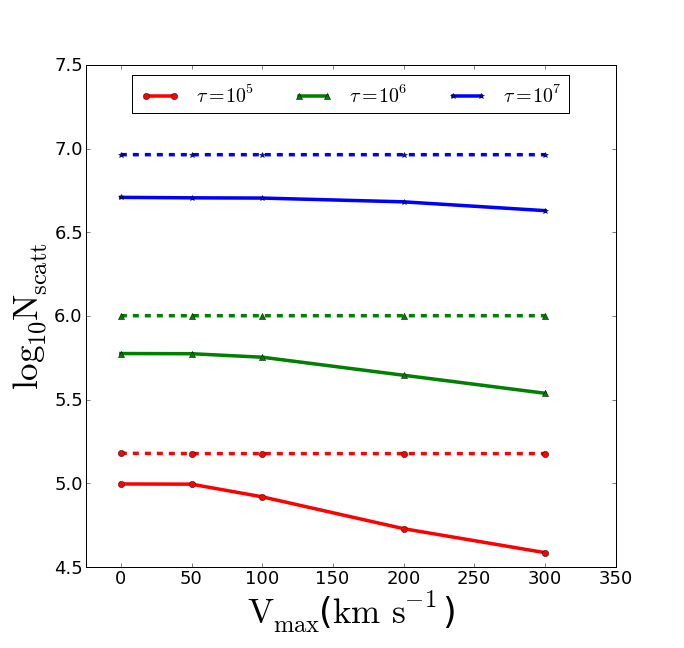
\includegraphics[width=0.45\textwidth]{NscattvsVmax.png}
\caption{Log of the Average number of scatterings of the outgoing
  photons as function of the velocity. \label{fig:Nscatt}}  
\end{figure}


\begin{figure*}
     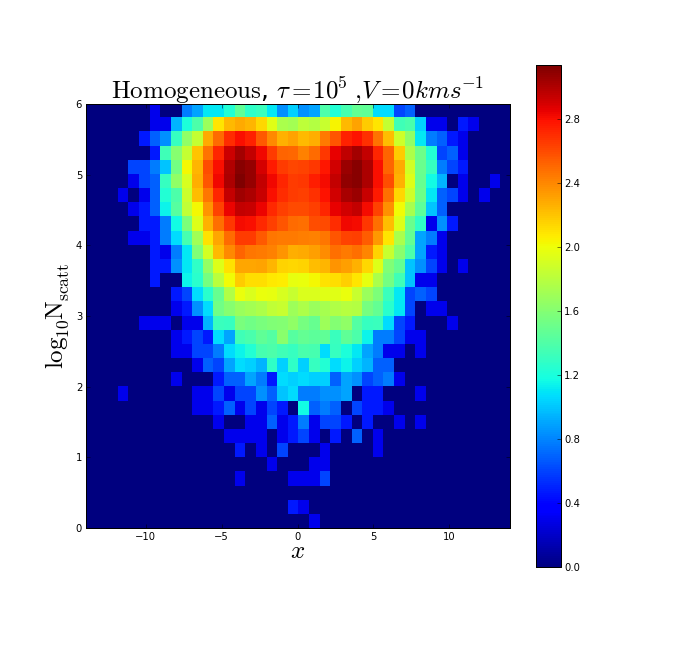
\includegraphics[width=0.40\textwidth]{2dHistogram0t5HOM.png}
     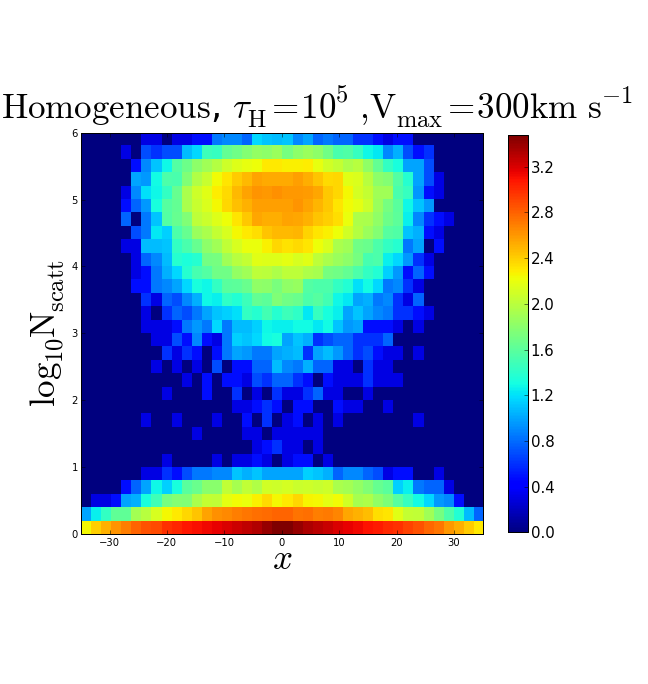
\includegraphics[width=0.40\textwidth]{2dHistogram300t5HOM.png}    
    \caption{Histogram of $N_{scatt}$ vs $x$ for the homogeneous
      distribution, left for $V_{max}=0km/s $, right for
      $V_{max}=300km/s$ \label{fig:NscattHistoHOM}}  
\end{figure*}

\begin{figure*}
     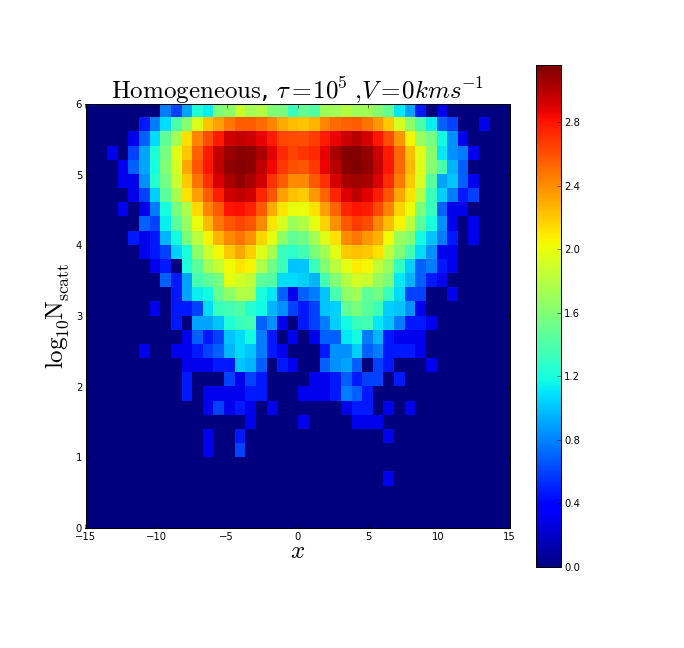
\includegraphics[width=0.40\textwidth]{2dHistogram50t5.png}
     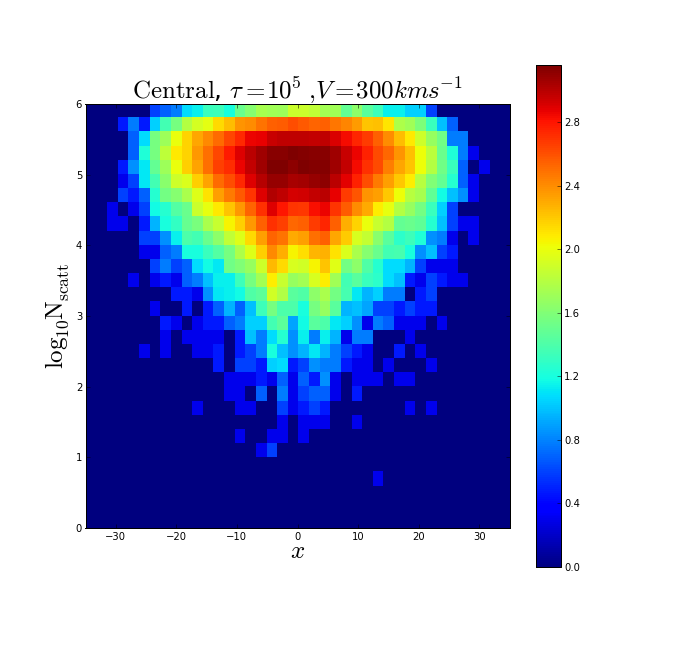
\includegraphics[width=0.40\textwidth]{2dHistogram300t5.png}    
    \caption{Histogram of $N_{scatt}$ vs $x$ for the Central
      distribution, left for $V_{max}=50km/s $, right for
      $V_{max}=300km/s$ \label{fig:NscattHistoHOM}}  
\end{figure*}


\subsection{Escape Fraction}
\label{sec:EF}

Until now we have studied models in absence of dust, but is known (REFERENCE) 
that there is presence of dust in high redshift galaxies. Our models with 
dust are treated as is explained in detail in  the appendix of (Forero et al 2011).  

Of particular interest is to compute the escape fraction of Lyman $\alpha$ 
photons coming from the most distant galaxies, due to the fact that with the 
observed intensity of the Lyman alpha line quantities as the LF and SFR can 
be derived (put some references).

Previous studies have shown the correlation of the Escape fraction with galactic 
mass (Laursen et al 2009, Dayal et al 2010) abundances and the kinematics of dust. 
In order to study pure rotational effects in the escape fraction we fixed the dust 
abundance $\tau_{A}=0.01$ and the galaxy mass. We compute the escape fraction for 
the models described in Table \ref{table:models}.

For a realistic model we also take into account the viewing angle, first we fixed 
the viewing angle at $\theta = 0$  Fig.~\ref{figure:efvsv} and then we fixed the 
velocity in order to see the escape fraction correlation with the viewing angle. 
Therefore we define the escape fraction as:\\ 

\begin{equation}
F_{e}=\dfrac{\Sigma_{NI} \vec{k}\cdot \vec{o}}{\Sigma_{NF}\vec{k}\cdot \vec{o}}
\end{equation}

Where NI is the initial number of photons and NF is the final,
$\vec{k}$ is the rotation axis direction and ${o}$ the observer
direction. With this definition we compute the escape fraction for all
of our models, the results are presented in Fig \ref{figure:efvsv}\\  
 
\begin{figure}
  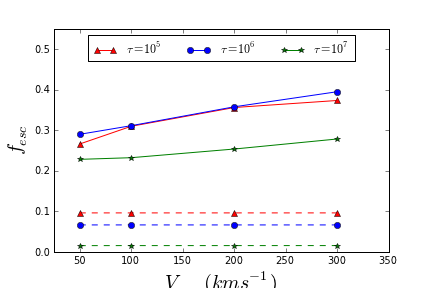
\includegraphics[width=0.45\textwidth]{EscapeFraction.png}
   \caption{Escape fraction for all the models. continious lines represent the homogenous models, while dashed lines represent the central models}\label{figure:efvsv}
\end{figure}

In Figure \ref{figure:efvsv} we found that in the central distribution
the escape fraction does not change with velocity while it does in the
optical depth (See Verhamme 2006, an argument about this). On the other
hand for the homogeneous distribution we
found that for higher velocities photons escape easily. The difference
between this two results rely in the fact that in the homogeneous
distribution photons are emitted closer to the escape surface and this
makes this configuration more sensitive to rotation while in the
central configuration the escape fraction depends mainly in the amount
of gas rather than in rotation. 

As a final test we compare our results with the analytical solution of 
the slab developed by (Neufeld 1990) Fig. ~\ref{figure:efvsNeufeld}, as 
the geometry we use is different from the one described for Neufeld, we 
dont expect the same results, in fact we found that for the homogenous 
sphere the escape fraction is higer than the slab (see ref, mark). Also 
we notest that for $\tau<10^{6}$ the escape fraction does not increase 
as it will be expected, This is due to the fact that the condition 
$a\tau_{h}>>\tau_{d}$ in not valid any more.


\begin{figure}
  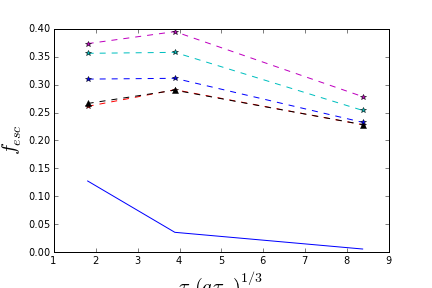
\includegraphics[width=0.45\textwidth]{Neufeld.png}
 \label{figure:efvsNeufeld}\caption{Escape fraction of this work
   compared with Neufeld analytical solution}  
\end{figure}

\subsection{The Case of Asymmetric Emission}

As we know there is unlikely to find galaxies with radiation sources 
distributed homogeneously. Most of them are in a clumpy distribution 
(Laursen et al 2013*) which affected the resulting spectra. In order 
to study an inhomogeneous distribution we set up a model in which we 
select certain photons that are placed in a specific place but that 
are not symmetrically distributed Fig.~\ref{figure:distributions} shows
the distributions we set up. 

\begin{figure}
  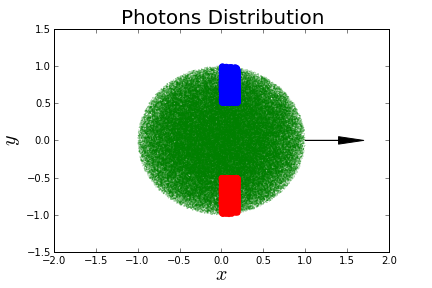
\includegraphics[width=0.40\textwidth]{Distribution.png}
  \caption{Inhomogeneous distributions of 
 photons, Blue area represents the photons in distribution 1 while red
 area are the selected photons for distribution 2. The arrow points to
 the observer position\label{figure:distributions}}  
\end{figure}

In Fig.~\ref{figure:inhomogeneous} we show the resulting spectra of 
distribution 1 and 2, the first effect we see is the asymmetry of the
double peak, in the homogeneous and central distribution we see double
peaks with the same height, while in this case one peak is higher than 
the other. For $\tau=10^{5}$ we found that in distribution 1 the blueshifted
peak is higher than the redshifted, and for distribution 2 the redshifted
peak is the highest.

An other important fact here is the asymmetry of the spectra with respect 
to the line center, in particular photons selected in distribution 1 
present a blueshift in their spectra while photons selected in distribution 
2 present a redshift. This effect becomes stronger as velocity increase 
~\ref{figure:inhomogeneous}
 
\begin{figure*}
  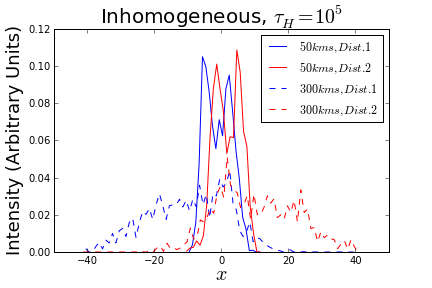
\includegraphics[width=0.45\textwidth]{InomogeneousModelt5.png}
  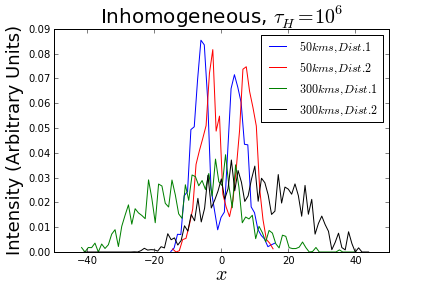
\includegraphics[width=0.45\textwidth]{InomogeneousModelt6.png}
 \caption{Inhomogeneous model for velocities $50km/s$ and $300km/s$ ,
   (left) with $\tau=10^5$, (right) with
   $\tau=10^6$\label{figure:inhomogeneous}}  
\end{figure*}
 

\subsection{Integrated flux in a narrowband filter}

Until now we have shown the main effects of gas and dust rotation in
the Ly$\alpha$ line morphology such as the escape fraction, the FWHM,
the maxima position, also we see that shape of the outgoing spectra
depends on the position of the observer. It is important to see if
rotational effects are detectable in observational methods involving
the Ly$\alpha$ line.  

One of the most used methods to detect high redshift galaxies using
the Ly$\alpha$ line is using a narrowband selection, we make this
analysis based on the results obtained by Steidel (2011) in this work
(EXPLAIN a lit of bit more about their work) they used tree narrowband
filters for tree different redshifts resumed in
Table~\ref{table:NBfilters}, We want to know how much the integrated
flux change due to rotational effects in this NB filters, for the
models we simulated with CLARA. 

\begin{table*}
\begin{center}
\begin{tabular}{cccc}\hline
Model & SSA22a 4980/80   & HS1549 4667/80 & HS1700 4018/90\\
\hline
\end{tabular}
\caption{
Fluxes for tree different narrow band filters.
} 
\label{table:NBfilters}
\end{center}
\end{table*}

In table \ref{table:NBfilters} we present the results of the flux in
every  narrowband filter for the homogeneous model at different
velocities and hydrogen  optical depth $\tau_{0}$. As is well known an
increase in the optical depth makes  the line peaks separation
bigger. In fact for some cases the line width is larger  than the NB
filer width fig.(put ref fig) for those cases we modify the redshift
in the available range in order to make the peak maxima match the NB
filter center.  For all cases we found that as velocity increase the
flux is less.  

In the case of the dusty model we found the same trend of the flux
with the velocity  but in this cases the effect is no that strong.  We
also found some dependency with the viewing angle. 

\begin{figure}
  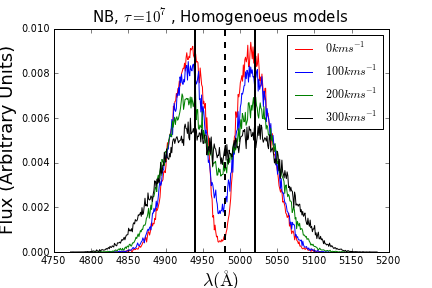
\includegraphics[width=0.45\textwidth]{NB7tDifVHOM.png}
 \label{figure:efvsNeufeld}\caption{NB filter located at the center of
   the maxima, with different redshift}  
\end{figure}

\section{Discussion}
\label{sec:discussion}

... Comparison with Verhamme et al. results on the rotation
... Compare with Kulas et al (Figure 3), Rotation on the lyman alpha
line convert double peak profiles into a single one. comments about
rotation with inflows and outflows.  

... The results derived in this paper have consequences on the
interpretation of galaxy observations in the Lyman alpha line.
..compare steidel et al (2011)
% taking into account equivalent widths results with narrow band
% filters we can make a criterium in order to select wich galaxie
% could be seen in actual observations.  



\section{Conclusions}
In this paper we have estimated the effects of gas bulk rotation on
the emission  of the Lyman $\alpha$ line. We based the study on the
study of a simplified configuration of an homogeneous sphere rotating
as a solid body. We explored  a range of models by varying the
rotation speed, hydrogen optical depth, dust optical depth and initial
distribution of Ly$\alpha$ photons with respect to the gas
density. This was implemented in CLARA, a Monte-Carlo
radiative transfer code already used to study the Lyman $\alpha$
line. 

As first we see how the width of the line changes using a modified FWHM
explained in section \ref{sec:widthpeak}, and we found that as gas bulk 
rotation increase also the width increase in a factor of $2-3$ in comparison 
with the static case. We also take into account the influence of the observer 
viewing angle, we found that observers with a line of sight perpendicular  
to the axis of rotation measure a $15\%$ larger line width than those 
aligned with the rotation axis.

As many observational spectra Ly$\alpha$ emission line (Kulas et al)
is double  peaked, these peaks provide important information
concerning gas kinematics and geometry,  which can be partially
explained with inflows/outflows of gas content.  We study the effect
of rotation in the position of this peaks, and we find  that the
position of the maxima does change with rotation for the homogeneous
models when the double peak merged into a single peak as velocity
increase. This effect is not seen for the central distribution when
the double peak  remains constant as the velocity increase. We also
find that there is no dependency in the observer viewing angle with
the maxima position. 

Concerning the escape fraction under rotational effects on the
Ly$\alpha$ emission line, we found that the escape fraction increase
in about $20\%-30\%$for the homogeneous sphere model. While rotational
effects are negligible for the central models and the escape fraction
remains constant. Also the observer viewing angle have no effect in
the escape fraction neither for the homogeneous and central
models. Complementing this analysis we study the average number of
scatterings $<N_{scatt}>$ that photons perform before escaping of the
cloud taking into account rotational effects. The main result here is
for the homogeneous models for which as velocity increase photons
escape with about $\sim 39\%$  less scatterings than in the static
case. 

As an application of these results we compute the integrated flux
taking into account the narrow band filters used by (Steidel et al
2011), for our models we found an important decrease up to $~40\%$ for
the homogeneous models, and up to $22\%$ for the dusty homogeneous
models in the flux as velocity increase.  Also we calculate at what
redshift should the filter be in order to get the maximum  flux, and
for the tree filters we get values that rely in the filter redshift
range. This effects would have a relevant implication at the time to
find high redshift galaxies.

This paper illustrates for the first time the main effects of rotation
in the morphology of the Ly$\alpha$ emission line, we estimate the
range of this effects for simplified models.


\section*{Acknowledgements}


\bibliography{references} 

\section*{Appendix A: Tables}


\end{document}



%ideas:
Keep in mind making a follow up paper on the results of Yamada et atl
http://adsabs.harvard.edu/abs/2012ApJ...751...29Y on the line
morphology at z=3.1. How many of t hese laes can be considered to have
rotation features? In principle, all of then should have them. How to
make the case convincing in the statistical sense? 

